%! Author = user
%! Date = 13.06.2023

\documentclass[a4paper, 14pt]{article}
%\documentclass[draft]{article}

\usepackage[T2A]{fontenc}
\usepackage[utf8]{inputenc}
\usepackage[english, russian]{babel}
\usepackage[top = 2cm, bottom = 2cm, left = 2cm, right = 2cm]{geometry}
\usepackage{indentfirst}
\usepackage{xcolor}
\usepackage{hyperref}
\usepackage{gensymb}
\usepackage{pgfplots}
\usepackage{amsmath, amsfonts, amsthm, mathtools}
\usepackage{amssymb}
\usepackage{physics, multirow, float}
\usepackage{wrapfig, tabularx}
\usepackage{icomma} % Clever comma: 0,2 - number while 0, 2 - two numbers
\usepackage{tikz, standalone}
\usepackage{fancyhdr,fancybox}
\usepackage{lastpage}
\usepackage{booktabs}
\usepackage{listings}
\usepackage{lstmisc}
\usepackage{stmaryrd}
\usepackage{amstex}

%\полуторный интервал
\onehalfspacing

\hypersetup
{   colorlinks = false,
    linkcolor = blue,
    pdftitle = {genphys},
    pdfauthor = {Володин Максим},
    allcolors = [RGB]{010 090 200}
}

\graphicspath{{./images/}}
\DeclareGraphicsExtensions{.pdf,.png,.jpg}

\restylefloat{table}
\usetikzlibrary{external}

\mathtoolsset{showonlyrefs = true} % Numbers will appear only where \eqref{} in the text LINKED
\pagestyle{fancy}

\fancyhf{}
\fancyhead[L]{Вопрос по выбору}
\fancyhead[R]{Реальный газ}
\fancyfoot[L]{}
\fancyfoot[R]{\thepage /\pageref{LastPage}}

\pgfplotsset{compat=1.18}

\begin{document}
    \begin{titlepage}
        \begin{center}
        {\large МОСКОВСКИЙ ФИЗИКО-ТЕХНИЧЕСКИЙ ИНСТИТУТ \\ \vspace{5mm}
        НАЦИОНАЛЬНЫЙ ИССЛЕДОВАТЕЛЬСКИЙ УНИВЕРСИТЕТ \\ \vspace{5mm}
        КАФЕДРА ОБЩЕЙ ФИЗИКИ}
        \end{center}

        \begin{center}
        {\large}
        \end{center}

        \vspace{5cm}

        {\huge
            \begin{center}
            {\textbf{Вопрос по выбору}}
                \\
                Модели реального газа
            \end{center}
        }

        \vspace{2cm}

        \begin{flushright}
        {
            Володин Максим \\
            \vspace{2mm}
            Б02 -- 206 \\
            \vspace{2mm}
            Физтех-школа физики и исследований имени Ландау
        }
        \end{flushright}

        \tableofcontents \vspace{2.5cm}

        \begin{center}
            Долгопрудный \\
            14 июня 2023 года
        \end{center}

    \end{titlepage}


    \section*{Реальный газ и его состояния} \addcontentsline{toc}{section}{Реальный газ и его состояния}

    Реальный газ — в общем случае — газообразное состояние реально существующего вещества.
    В термодинамике под реальным газом, понимается газ, частицы которого имеют кинетическую и потенциальную энергии
    взаимодействия между собой.
    Этот газ не описывается в точности уравнением Менделеева — Клапейрона, в отличие от его упрощенной модели —
    идеального газа, в котором взаимодействие частиц друг с другом мало.
    Данная модель хорошо работает с высоко перегретыми газами, однако на температурах $10^3 K$ и ниже состояние газов
    заметно отличается от идеального.
    Стоит отметить, что, например, насыщенный пар (двухфазовая равновесная система жидкость — пар), вообще не
    подчиняется законам идеального газа, несмотря на то, что ещё в школе были попытки описать его таким образом

    Далее предлагается рассмотреть различные уравнения реальных газов


    \section*{Модель Ван-дер-Ваальса} \addcontentsline{toc}{section}{Модель Ван-дер-Ваальса}

    Модель газа Ван-дер-Ваальса является одной из самых простых и самых распространенных моделей реального газа при
    изучении.
    Итак, в модели идеального газа взаимодействие между молекулами газа отсутствует.
    Однако в реальности, даже если газ состоит из электрически нейтральных молекул, они все-таки взаимодействуют друг
    с другом.
    На больших расстояниях между молекулами возникают силы притяжения.
    Эти силы называются силами Ван-дер-Ваальса.
    Связано это с тем, что внутри атома или молекулы центры положительных и отрицательных зарядов не совпадают в
    одной точке, что приводит к наличию вокруг атома электрического поля.
    Возникает поляризация молекул, а полярные молекулы уже взаимодействуют друг с другом

    Если расстояние между молекулами велико по сравнению с их размерами, то такие силы взаимодействия - это силы
    притяжения.
    Они убывают обратно пропорционально седьмой степени расстояния.
    На близких расстояниях электронные оболочки взаимодействующих молекул начинают перекрываться, и силы
    молекулярного притяжения переходят в силы отталкивания, которые растут с уменьшением расстояния как

    Потенциальная энергия взаимодействия двух нейтральных молекул описывается потенциалом Леннард-Джонса:
    \[ \Pi (r) = \frac{A}{r^{12}} - \frac{B}{r^6} \]
    Константы $A, B$ являются характеристиками атомов вещества.
    Соответствующая ему потенциальная сила взаимодействия имеет вид
    \[ F(r) = - \frac{12A}{r^{13}} + \frac{6B}{r^7} \]

    Изобразим этот потенциал на Рис~\ref{6-12}.
    На этом же рисунке штриховой линией показана аппроксимация взаимодействия молекул, примененная в модели
    Ван-дер-Ваальса.
    Кривая в области отталкивания заменена на вертикальную прямую, отстоящую от $r = 0$ на величину диаметра $d$
    молекулы.
    Ближе расстояния $d$ молекулы сойтись не могут, потому что в модели Ван-дер-Ваальса используется модель молекул
    как твердых упругих шариков

    \begin{figure}[h]
        \begin{center}
            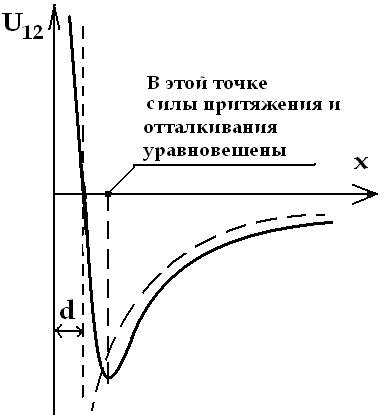
\includegraphics[width = 0.5 \textwidth]{6-12}
            \caption{Зависимость потенциальной энергии от расстояния между молекулами}\label{6-12}
        \end{center}
    \end{figure}

    Здесь не приводится вывод уравнения Ван-дер-Ваальса, потому как для этого есть отдельный билет.
    Стоит отметить, что данная модель имеет точность порядка $25 \%$ (сравнение с экспериментальными данными).
    За создание и исследование данной модели Йоханнес Дидерик Ван-дер-Ваальс был прижизненно удостоен Нобелевской
    премии по физике


    \section*{Модель Дитеричи} \addcontentsline{toc}{section}{Модель Дитеричи}

    Влияние пристеночного молекулярного слоя на уравнение состояния можно учесть и по-другому.
    Пусть молекулярная стенка действует на молекулы газа только при столкновении с ними.
    Молекулы пристеночного слоя подвергаются действию результирующей силы, направленной внутрь газа.
    Вследствие этого концентрация молекул в пристеночном слое должна убывать при приближении к стенке в соответствии с
    формулой Больцмана: $n = n_w e^{-\frac{U}{kT}}, $ где $U$ - потенциальная энергия молекулы.

    Этим и объясняется уменьшение давления газа на стенку.
    Энергия $U$ - функция расстояния $x$ молекулы от стенки: $U = U(x)$.
    Она максимальна у самой стенки и быстро убывает с возрастанием $x$.
    Ее значение на бесконечности будем считать равным нулю.

    Давление на стенку определяется пристеночной концентрацией $n_w$.
    Вновь считая молекулы точечными, можем написать

    \begin{equation}
        \label{eq:P}
        P = n_w kT = n_w kT e^{-\frac{U_w}{kT}},
    \end{equation}

    где $U_{w}$ - значение потенциальной энергии молекулы у стенки сосуда.

    Если выполнено условие $U_w \ll kT$ (у стенки молекулы не двигаются), то $e^{-\frac{U_w}{kT}} \approx 1 -
    \frac{U_w}{kT}$ (разложение по формуле Тейлора).
    Тогда получим следующее:

    \[ P + n_w U_w = n_0 kT \]

    Из этой формулы видно, что сила притяжения, действующая на пристеночную молекулу, а с ней и потенциальная энергия $
    U_w$, пропорциональны концентрации молекул газа $n_0 = \frac{N}{V}$.
    Поэтому можно написать $U_w = \alpha n_0$, где $\alpha$ -- некоторая постоянная величина.
    Тогда предыдущая формула преобразуется к виду

    \[  \left(P + \alpha n_0^{2} \right) = n_0 kT \\
    \Leftrightarrow (a = \alpha N^2, PV = RT) \Leftrightarrow \\
    \left(P+\frac{a}{V^{2}}\right)V = RT                        \]

    С помощью введённой постоянной $a$ выразим потенциальную энергию:

    \begin{equation}
        \label{eq:u_w}
        U_w = \frac{a}{NV}
    \end{equation}

    Вернемся к формуле~\eqref{eq:P}, но уже не будем аппроксимировать показательную функцию линейной.
    Тогда с учетом~\eqref{eq:u_w} получим:

    \[ P = n_0 kT \exp \left( -\frac{a}{RTV} \right) = \frac{RT}{V} \exp \left( -\frac{a}{RTV} \right) \]

    Учтём конечный объем молекул:

    \[ \mathrm{P}(V - b) = RT \exp \left( -\frac{a}{RTV} \right) \]

    Данное уравнение и есть уравнение Дитеричи.
    Стоит отметить, что в предельном случае, когда $b \ll V$ и $a \ll RTV$, уравнение Дитеричи переходит в уравнение
    Ван-дер-Ваальса.
    Это достигается за счёт аппроксимации показательной функции в формуле Дитеричи линейной

    \section*{Модель Бертло} \addcontentsline{toc}{section}{Модель Бертло}
    Уравнение Бертло -- это еще одна модификация газа Ван-дер-Ваальса, опубликованная в 1899 году.

    Бертло предположил, что коэффициент $a$ уравнения Ван-дер-Ваальса имеет вид $a = \frac{a^{\prime}}{T}$.
    Тогда новое уравнение будет иметь вид:

    \begin{equation}
        \label{eq:Berthelot}
        \left(P + \frac{a^{\prime}}{TV^{2}} \right)(V-b) = RT
    \end{equation}

%    Найдём эту постоянную $a^{\prime}$; данный процесс аналогичен процессу нахождения критических параметров
%    В критических точках первая и вторая производные от давления по объему при постоянной температуре равны 0, причем
%    такая точка является единственной.
%    Выразим давление из формулы~\eqref{eq:Berthelot}:
%
%    \[ P(V) = \frac{RT}{V - b} - \frac{a^{\prime}}{TV^2} \]
%
%    Возьмем производную $\frac{\partial P}{\partial V}$ и подставим критические значения для температуры и объема.
%    Получим
%
%    \[
%        \frac{\partial P}{\partial V} = -\frac{RT_{cr}}{\left(V_{cr} - b\right)^{2}} + \frac{2 a^{\prime}}{T_{cr}
%            V_{cr}^{3}} = 0 \\
%        a^{\prime} = 3 P_{cr} T_{cr} V_{cr}^{2}
%    \]

    \section*{Модель Камерлинга-Оннеса} \addcontentsline{toc}{section}{Модель Камерлинга-Оннеса}

    Нидерландский физик и химик Хейке Камерлинг-Оннес предложил уравнение состояния полуэмпирического типа, которое
    имеет следующий вид:

    \[ PV = A + \frac{B}{V} + \frac{C}{V^2} + \frac{D}{V^4} + \frac{E}{V^6} + \frac{F}{V^8} \]

    Стоит отметить, что данное уравнение учитывает все особенности реальных газов в наиболее полном виде

    Коэффициент $A$ определяется как $A = RT$.
    Коэффициенты $B, C$ и последующие называются вторым, третьим и так далее вириальными коэффициентами.
    Они так же как и в модели Бертло являются функциями температуры:

    \[ B = b_1 + \frac{b_2}{T} + \frac{b_3}{T^2} + \frac{b_4}{T^4} + \frac{b_5}{T^6} \]

    Стоит отметить, что уравнение всякого газа может быть приведено к виду формулы Камерлинга-Оннеса.
%    Но данное уравнение приобретает конкретное содержание только после того, как будут найдены выражения для всех
%    входящих в него вириальных коэффициентов (чаще всего, это делается экспериментально)

    \section*{Область применимости моделей} \addcontentsline{toc}{section}{Область применимости моделей}

    Мы убедились, что существует множество уравнений, с помощью которых люди пытались описать модель реального газа
    максимально точно.
    За счет увеличения эмпирических постоянных, входящих в эти уравнения, удается достигнуть лучшего согласия с
    опытом по сравнению с тем, что дает уравнение Ван-дер-Ваальса.
    Уточним эти слова ниже

    \subsection*{Модель Ван-дер-Ваальса} \addcontentsline{toc}{subsection}{Модель Ван-дер-Ваальса}

    Модель Ван-дер-Ваальса остаётся самым распространенным благодаря своей простоте и ясному физическому
    смыслу входящих в него постоянных.
    Оно правильно описывает явления, связанные с изменением плотности газов при изменении температуры и давления,
    взаимные переходы жидкости и газа.
    Из уравнения Ван-дер-Ваальса вытекает наличие у веществ критической точки.
    В то же время модель Ван-дер-Ваальса имеет существенные недостатки

    Во-первых, параметры $a$ и $b$, входящие в уравнение Ван-дер-Ваальса не являются до конца постоянными.
    Они хоть немного, но зависят от температуры, хотя по смыслу уравнения Ван-дер-Ваальса $a$ и $b$ должны быть
    постоянными, характерными для данного вещества величинами

    Во-вторых, существует количественное расхождение между теоретическим уравнением и опытом по нахождению
    критических параметров $T_{cr}, V_{cr}, P_{cr}$
    Было установлено, что между этими величинами должно существовать соотношение $\frac{T_{cr}}{P_{cr}V_{cr}} =
    \frac{8}{3}R$.
    Опыт же показывает, что хотя величина постоянна для многих веществ, но равна аж $3,7 R$.
    Вместо вытекающего из уравнения Ван-дер-Ваальса соотношения $V_{cr}=3 b$, опыт показывает, что значительно лучше
    выполняется равенство $V_{cr} = 2b$.

    Таким образом, уравнение Ван-дер-Ваальса правильно описывает явления только качественно, по порядку величины.
    Для количественных оценок оно является грубым

    \subsection*{Модель Дитеричи, Бертло и Камерлинга-Оннеса} \addcontentsline{toc}{subsection}{Модель Дитеричи и
    Бертло}

    Уравнение Дитеричи для умеренных давлений значительно лучше уравнения Ван-дер-Ваальса, но совершенно непригодно
    для больших давлений, как и уравнение Ван-дер-Ваальса

    Результаты опытов показали, что уравнение Бертло хорошо работает и согласуется с опытами при давлениях около 5 -- 6
    атмосфер и температурах выше критической, очень низких температурах и в области низких давлений.
    Данное уравнение достаточно точно описывает свойства газов небольшой плотности, имеющих температуру кипения от
    $700 \celsius$ до $2000 \celsius$, то есть это такие газы, как водород, аргон, кислород и другие.
    В критической области и больших давлениях уравнение Бертло неприменимо

    Уравнение Камерлинга-Оннеса наиболее точно описывает реальные газы, учитывая их свойства
    и особенности.
    Однако и у него есть некоторые недостатки, например, из-за достаточно большого количества так называемых вириальных
    коэффициентов осложняется процесс нахождения этих величин.
    Так как каждый из данных коэффициентов от температуры процесс нахождения каждого из них становится достаточно
    времязатратным
%
%    \begin{thebibliography}{}
%        % \addcontentsline{toc}{chapter}{\bibname}
%        \bibitem{1} Бутиков Е.\ И., Кондратьев А.\ С. Физика для углублённого изучения.\ Книга 3.\ Строение и свойства
%        вещества -- М.: Наука, 1994.\ — 367 с.
%        \bibitem{2} [Источник изображений] \href{https://textarchive.ru/}{Банк научно-популярных статей textarchive}.
%        Режим доступа -- свободный.\ Дата обращения -- 13.06.2023.
%    \end{thebibliography}

\end{document}